\appendix{}
\gdef\thesection{Appendix \Alph{section}}

\section{Figures}
\label{sec:figures}

\begin{figure}[htbp]
  \centering
  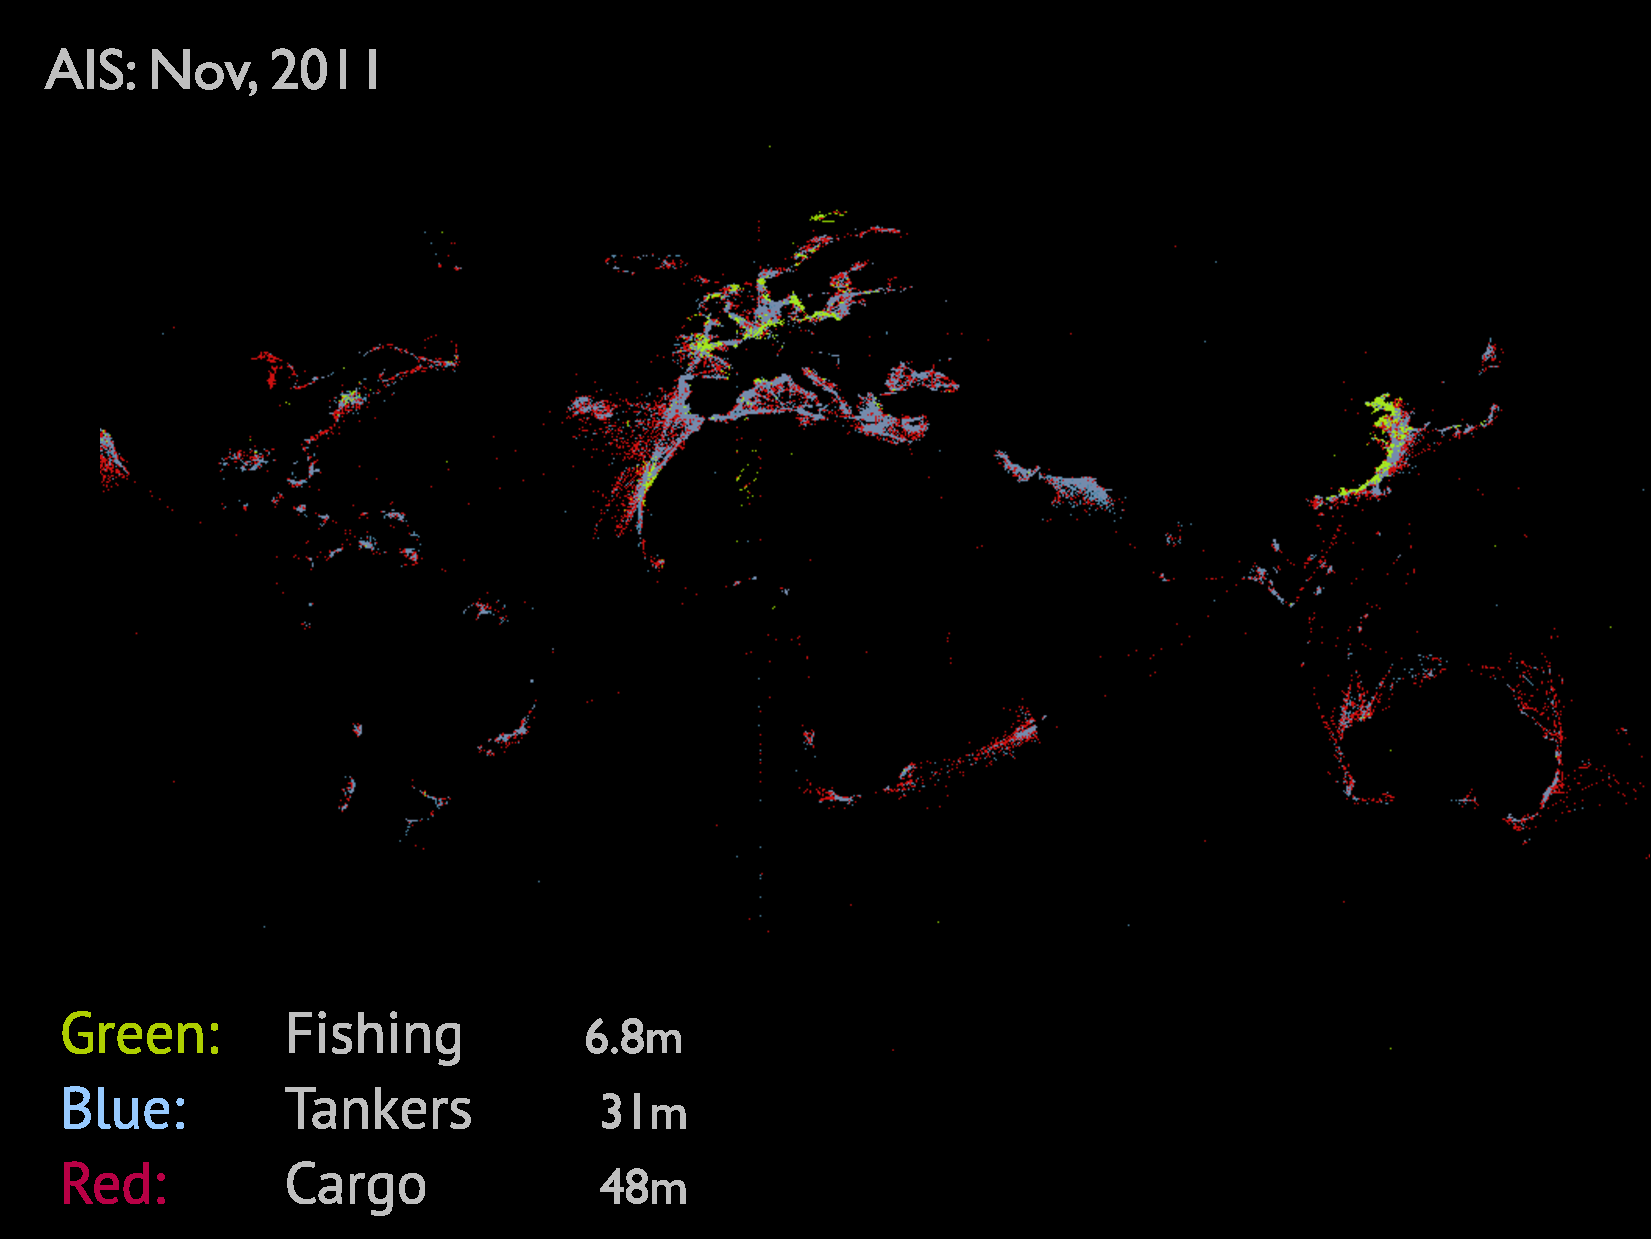
\includegraphics[width=160mm]{figures/ais-nov-2011.pdf}
  \caption{Raw AIS observations, November 2011. Note the observations located in the Hoggar Mountains in Algeria.}
  \label{fig:ais-obs-nov-2011}
\end{figure}

\begin{figure}[htbp]
  \centering
  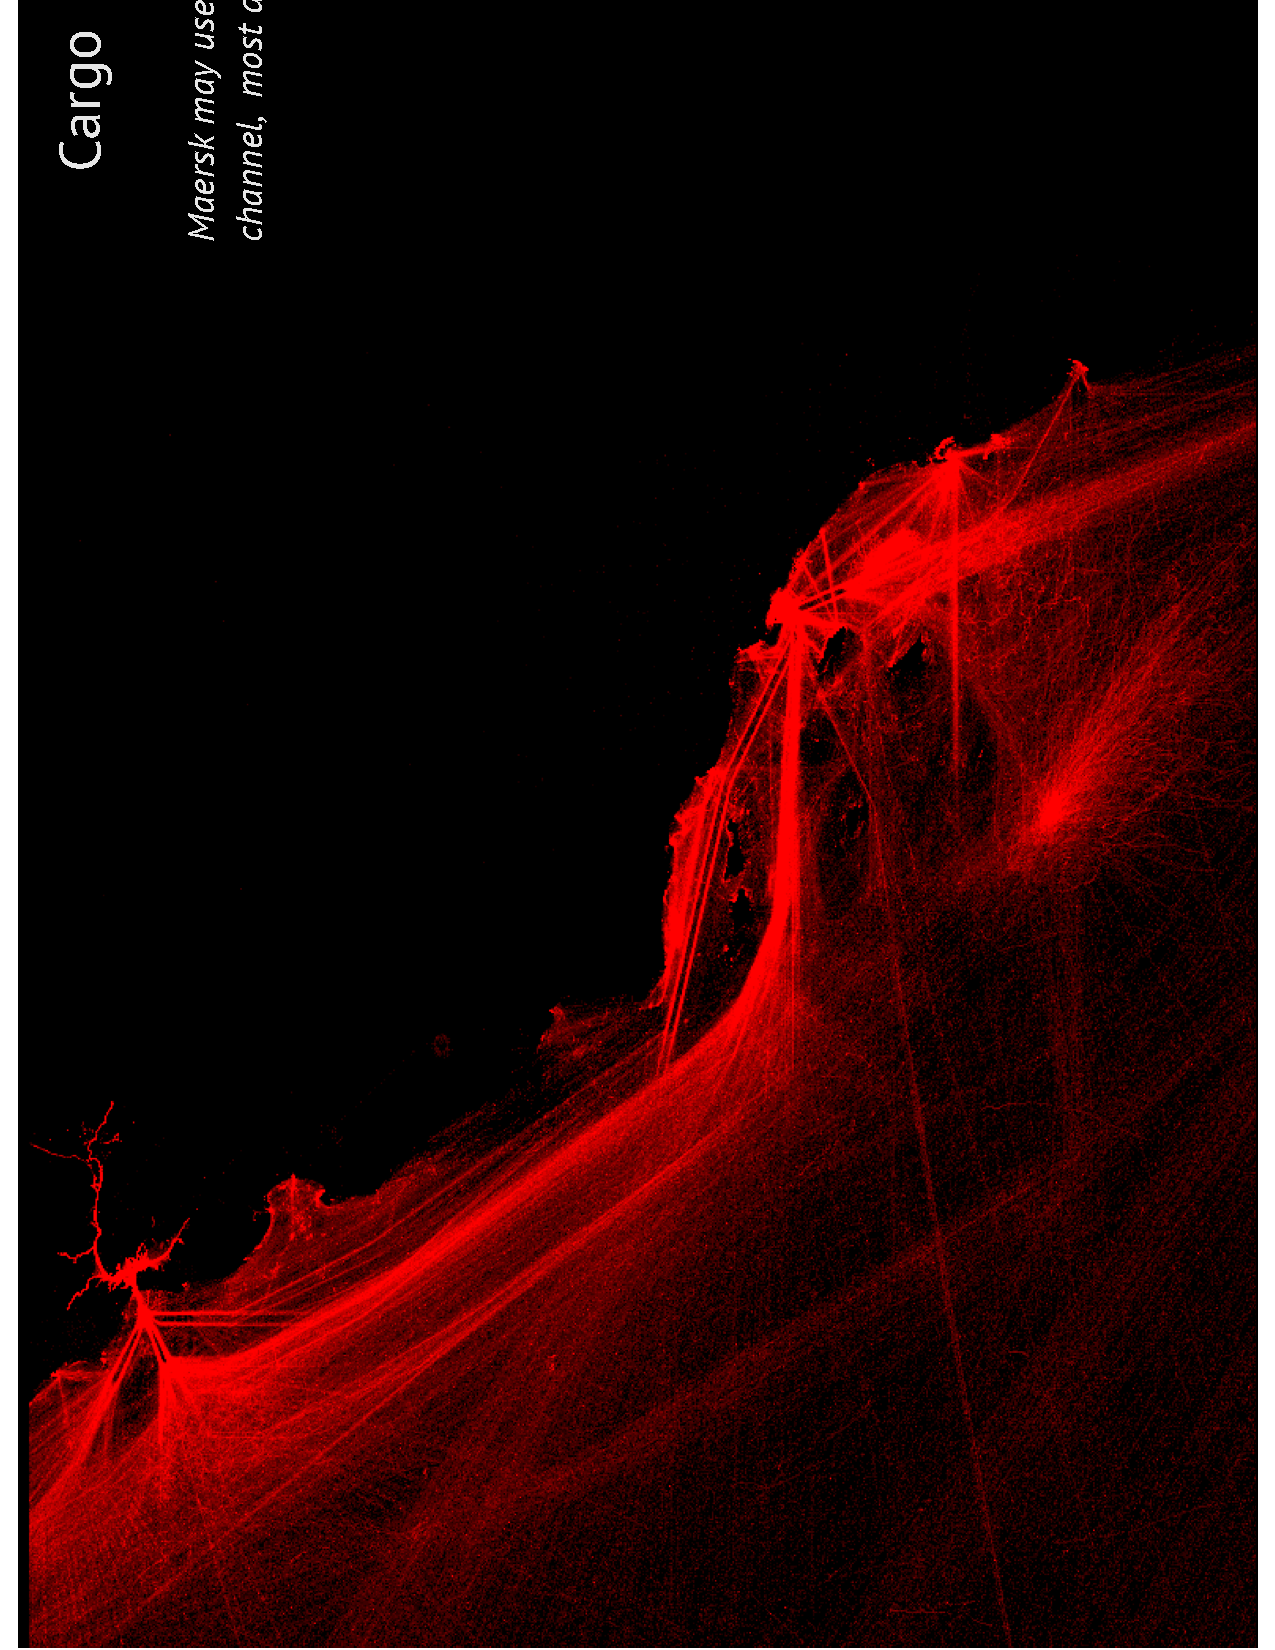
\includegraphics[width=140mm,angle=-90]{figures/cal-cargo.pdf}
  \caption{AIS observations, Southern California Bight. Nov 2011--Dec 2012. Note the ballast water exchange point lower left.}
  \label{fig:cal-cargo}
\end{figure}


\begin{figure}[htbp]
  \centering
  \includegraphics[width=160mm]{figures/ais-and-ports-cea.pdf}
  \caption{Approximate AIS coverage (green), global ports (red). Cylindrical Equal-Area projection}
  \label{fig:ais-coverage}
\end{figure}

%\section{Tables}

\begin{table}[htbp]
  \begin{tabular}{lr}
    Attribute & Accuracy \\
    \hline
    Location (fixed from GPS signal) & $\simeq$10 meter accuracy) \\
    Timestamp (on broadcast) & $\simeq$100 ms \textit{radio transmission \& processing latency}\\
    Name \\
    Call Sign \\
    Maritime Mobile Service Identity (MMSI) \\
    Heading \\
    Speed \\
    Destination & \textit{rarely valid}
  \end{tabular}
  \caption{AIS broadcast attributes. Update frequency depends on ship speed, but varies between a minimum of a record every 2 seconds for quickly moving vessels, to once per 3 minutes for moored vessels. Additional attributes are available, but infrequently used.}
  \label{table:ais-broadcast-attributes}
\end{table}

\newpage

\section{Source Code}
\label{sec:source-code}

% include SOME python code here -- our AIS parser, what else?
% steps: download AIS
% parse ais
% insert AIS into DB, formalize
% download & parse ship databases

\texttt{aiskml.py}:
\inputminted[linenos,
             numbersep=5pt,
             frame=lines,
             framesep=2mm]{r}{../code/kml/aiskml.py}

\texttt{parsekml.py}:
\inputminted[linenos,
             numbersep=5pt,
             frame=lines,
             framesep=2mm]{r}{../code/kml/parsekml.py}


